\section{Implementation on SLang}
\label{sec:implementation_slang}

In the implementation on SonarJava, we had access to the front end of the checker, with complete language, a control flow graph and the symbol resolution already present.
The first step to implement it on \slang{} is to identify what nodes and structure we need in order to implement everything that is required for this check.

\subsection{Nodes}
\label{subsec:nodes}

The particularity of \slang{}  is that it is incomplete. 
The IR does not need to includes all node types in order to work, only the one needed for the rules are mapped. 
We therefore have to make sure that we have all the nodes that we need in \slang{} for the implementation of the checker.

\begin{table}[h]
	\caption{All nodes needed for the null pointer dereference check}
	\label{table:nodes-needed}
	\begin{tabular}{|c|c|c|}
		\hline
		\bf Checker specific & \bf Needed for CFG & \bf Others  \\ \hline
	    Binary operation & If/else & Variable declaration \\
		Identifier & Switch & Function invocation \\
		Assignment & Exception handling, throw  & Function declaration \\
		Litteral : Null & Loops & Class declaration \\
		Member select & Jump (break, continue, …) & \\ \hline
	\end{tabular}
\end{table}

Table \ref{table:nodes-needed} shows the nodes that we need in order to implement the different parts of the checker.
The first column lists the nodes needed to recognize the different structures used in the checker. 
We can see that the list is quite simple. 
The interesting node is the member select, in fact, to identify when a pointer is used, we will only use this node: we don’t need to know anything about the context in which the pointer is used. 
For example, when a function is called without a member selection, the tree will simply be a identifier (name of the function) and a list of argument, but in the case of a pointer use, the tree will be a member selection, that we will use in the checker. 
This way, we are able to detect not only function invocation, but also field selection or anything that we consider as a member selection in the original language.

The nodes needed for the control flow graph are the one that we can expect for identifying the control flow of a program, that are common in all language and already implemented in \slang{}. 
The way we handle them will be described in subsection \ref{subsec:cfg_on_slang}.
The last column describes others nodes that are needed indirectly by the checker.

\subsubsection{Variable declaration}
\label{subsubsec:variable_declaration}

\lstinputlisting[label={lst:local-scope-in-while},
caption=Example of local scope inside a loop that can shadow field]{code/local-scope-in-while.scala}

In section \ref{subsubsec:identifying_local_variable}, we are going to describe how we perform a naive semantics, that is assumed inside the rule.
In this semantics, we are not going ot be able to differentiate if two pointer that have the same name refer to the same declaration. 
The idea to better support this limitation is that we will kill the pointer in the analysis when we see a declaration, the same way we are killing it when we see an assignment.
This will enable us to remove the kind of false positive of listing \ref{lst:local-scope-in-while}.

\subsubsection{Function invocation}
\label{subsubsec:function_invocation}

\lstinputlisting[label={lst:function-invocation-support},
caption=Pointer p is used as a parameter of a function call]{code/function-invocation-support.scala}

As discussed before, we do not need explicitly function invocation, only member selection. 
Due to a specific way we handle nodes that are not translated that we will explain in section \ref{subsec:how_to_deal_with_native}, we will add function invocation to be able to report pointer use that happens inside a function call, as illustrated in listing \ref{lst:function-invocation-support}.

\subsubsection{Function and Class declaration}
\label{subsubsec:function_class_declaration}

As our checker is only ran inside functions, we need function declaration to have our starting point. 
We also use this to improve our semantics, using the fact that the variable that is used inside a nested function is not checked.

Class declaration is used for the same idea as the function declaration, we use the assumption that variable declared in nested class are in an other scope.


\subsubsection{Other nodes not supported}
\label{subsubsec:other_nodes_not_supported}

In \ref{subsec:other_way_to_add_belief}, we saw multiple way to add the belief that a null pointer can be raised. 
Slang do not have arrays, so we could expect to not find all issues coming from them. 
The first is the length of the array. In Slang, this is simply represented as a field access/member select, and can therefore be supported. 
Accessing or modifying the slots of \emph{null} as if it were an array is however not supported. This will lead to false negative in \slang{} that we will not have in the implementation of SonarJava.

\subsection{Building a Control Flow Graph on SLang}
\label{subsec:cfg_on_slang}

\slang{} already have every control flow statements represented in the language, we can already start to build it the same way we would do it for any other language. 
In fact, the current implementation is greatly inspired by the implementation of the graph builder of SonarPHP \cite{SonarPHP:2019:Online}, also developed at SonarSource. 
To build the control flow graph, we are going to use two main kind of basic blocks:

\begin{enumerate}
	\item \textit{CFG Block} \newline 
	This is the base of all basic block of the graph, it contains the following fields:
	\begin{enumerate}
		\item \textit{Predecessors} \newline
		Nodes that may be executed \textbf{before} the current block.\newline
		\item \textit{Successors} \newline
		Nodes that may be executed \textbf{after} the current block.\newline
		\item \textit{Elements} \newline
		List of instruction that are executed one after the other in this basic block. \newline
		\item \textit{Syntactic Successor} \newline
		Node following the current block if no jump is applied. 
		This is not directly needed for any control flow graph, but it is sometimes required by some check that we may implement in the future.\newline
	\end{enumerate}
	\item \textit{CFG Branching Block} \newline 
	This interface represents blocks that include branching instruction, where the flow depend on the result of a Boolean expression. 
	It inherits from CFG Block and simply have a true and false successor block reference in addition to the simple block.
	\newline 
\end{enumerate}

Since we are going to build a graph for the content of a function, our starting point will be the list of the elements of the function.
We are going to start to build the graph from the end of the execution, using a bottom-up approach. It enables us to always know the successor of the node that we are currently building, making easier to build the different instructions that contains control flow.
We start by creating an END node, that contains no element and represents the end of the execution. We will then recursively build the graph by matching on the type of the tree.

\subsubsection{Block and others nodes}
\label{subsubsec:block_and_others}

The simplest tree that we will face are the blocks, they represent simply a list of statements, we can therefore directly recursively build the graph for all children. 
This behavior can also be applied to other known trees that does not change the flow of execution, as a default case. 
The only difference is that we are also going to add the current tree to the elements after having built the graph for the children, in order to not lose information. 
For example, having a list of identifier is not useful if we do not know that they are linked together by a binary expression, we will therefore add both the binary expression and the children to the elements of the current block.

\subsubsection{If/Then/Else}
\label{subsubsec:if_then_else}

This is the typical example that implements a branching block. 
We will first build the sub flow for the false and true branch, if present, and then construct a branching block with these two new blocks as successor. 
We can now recursively build the condition of the If tree from the branching block created before.

\subsubsection{Loops : For, While, Do-While}
\label{subsubsec:loops_cfg}

The bottom-up approach makes the creation of the If tree straightforward, since we have already built the successor of the tree that we are currently building. 
However in the case of loops, the flow is not going to continue at the successor, but return at the condition of the loop, a predecessor’s node that we have not built yet. 
To solve this issue, we can introduce a \textbf{forwarding block}, a simple basic block that is used to store a reference and will not contain any element. 
We can now start to build the loop flow by creating a forwarding block that will link to the condition, and build the body with this new block as the successor. 
Finally, we can build the condition of the loop as a branching block, with the true successor as the body of the loop, and the false as the block that follow the loop.
There is one details that we have not address yet: break and continue. 
To support these two statements, we are going to use a stack, that will contain breakable objects. These objects are simply here to store the link to the condition for continue, and the end of the loop for break. 
Before starting to build the body of the loop, we will push a breakable to the top of the stack, and pop it once we are done. 
The stack is used to support nested loop, a break/continue will refers to the first enclosing loop.

The current implementation of For loops is the same as While loops, this may introduce problems that will be discussed later. We can use the same idea for Do/While loop, and simply start to build the condition before the body.

\subsubsection{Match Tree}
\label{subsubsec:match_tree_cfg}

The particularity of a match tree is that it can behave differently depending on the original language. 
For example in Scala, only one match case can be executed, while in java, all cases are executed after a matching pattern, until a break. 
The second example is typically known as fallthrough. 
In Slang, both of them are mapped to the same node, however, identifying which one is the right behavior can be done by storing a flag in the node. 
Non-fallthrough match tree is an easy case, we can build all the cases separately, and create a block that will have multiples successors.

Fallthrough switch is more tricky, we first have to use the same idea as we used for loops: add a breakable to the stack, to store the reference to the block that is executed after the switch. 
We make the same assumption as we did with loop, that a break refers only to the closest enclosing switch. 

We are going to start by creating a forwarding block for the default case, and build the different cases, in the reverse order and one after the other. 
We create one branching block per match cases, with the body of the case as true successor and the next pattern as the false successor. 
At the same time, we build the sequence of the body of cases, starting from a break.

\lstinputlisting[label={lst:pattern-match},
caption=Example of pattern matching in Scala]{code/pattern-match.scala}

\begin{figure}[h]
	\caption{Corresponding CFG of the code of listing \ref{lst:pattern-match}}
	\label{figure:pat-mat-cfg}
	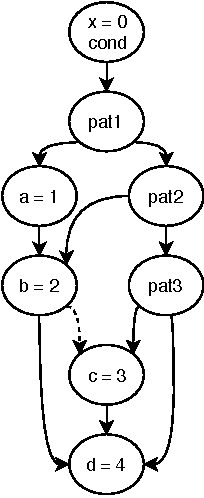
\includegraphics[]{figure/pat-mat-cfg.pdf}
\end{figure}



Figure \ref{figure:pat-mat-cfg} shows the resulting control flow graph of the code of listing \ref{lst:pattern-match}. We can see that the fallthrough behavior is represented as expected, \emph{a = 1} is executed both when \emph{pat1} and \emph{pat2} is true.

\subsubsection{Jump Tree: break and continue}
\label{subsubsec:jump_tree_cfg}

Jump tree are not supposed to appear when we do not expect them, if we have an unexpected jump tree, we can not do anything and we will simply add it to the current block. 
We will discuss in section \ref{subsec:how_to_deal_with_native} a solution to better support this situation.
In the usual case, we will expect them and create an edge from the current block to the head of the stack that is filled as described in \ref{subsubsec:loops_cfg} and \ref{subsubsec:match_tree_cfg} sections.

\subsubsection{Return}
\label{subsubsec:return_cfg}
Once again, starting from the end greatly simplify the support of return statements: we can store a reference to the \emph{END} block that is created at the beginning, use it as successor to the block that will contain the return expression.

\subsubsection{Exception Handling Tree and Throw Tree}
\label{subsubsec:exception_handling_cfg}
In our control flow graph, we are only going to consider exception that are explicitly thrown with a throw statements, and not add an edge to every statements where an exception can occur in reality. \newline
We are going to start at the end of the exception handling tree. 
When an exception handling tree is executed, it can results in two possible cases: the exception is catched and the flow can continue, or it is not and the flow goes to the end of the function. 
To support this behavior, we are going to create a block with two successor: the \emph{END} node recovered the same way we did for return statements and the successor previously created. \newline
We can then create the finally block, if present, and the different catch case separately, and continue to build the body of the try block. 
At this point we have to know where to jump in the case where an exception is thrown. 
To do this, we will use the same idea as we did with the jump trees: use a stack to push the target of the throw before building the body, and popping it after. 
If there is no catch block, the target will be the finally block, if there is one or more catch block, we will use the first catch case as target. 
This is an approximation that is due to the fact that we have no symbol resolution, we can not know which of the exception is catched or not. 
From now, we can know where to jump in the case of a throw three.\newline
The last detail to take care of is the case where we have a return inside an exception handling tree. 
In this case, the finally block is executed after the return. 
To support this, we will store the exit target on a stack, pushing the reference to the finally block on top of the \emph{END} block previously added.

\subsubsection{Natives Nodes}
\label{subsubsec:native_nodes_cfg}

The main challenge comes from the only new nodes that we have compared to any language: the \emph{natives nodes}. 
The way we deal with native nodes will be described in subsection \ref{subsec:how_to_deal_with_native}.

\subsubsection{Normalization}
\label{subsubsec:normalization_cfg}
The core of the graph is done, but we still need to perform a few modification in order to have a proper control flow graph. 
First, we are going to remove empty blocks. 
They can be introduced in multiple situations, when we create a temporary forwarding block or when the header of a for loop is empty for example.
During the creation of the graph, we only knew the successors of the nodes, we still have to compute the predecessor set. 
Since we have all successors, computing the predecessor of all the block is straightforward. Finally, we can create a \emph{START} node, that implements the same behavior as the \emph{END} node, to indicate the beginning of the flow. \newline
The hard work is done, we now have a complete control flow graph. 
There is still part of it that can be imprecise due to the fact that the different statements of the original language can behave differently, but we are going to discuss it later in section \ref{subsec:how_to_deal_with_native}.

\subsection{Data flow analysis}
\label{subsec:data_flow_analysis}

Now that we have all nodes needed and a control flow graph, we can start the implementation of the checker, that is in fact really similar to the one described in \ref{sec:implementation_java}. 
The main difference is the the way we deal with “unreliable” nodes and the identification of local variable. 
The former will be described in \ref{subsec:how_to_deal_with_native} and the latter in the next section.

\subsubsection{Identifying local variable}
\label{subsubsec:identifying_local_variable}

In SonarJava, we have access to symbols of identifier, information that we do not have in \slang{}. The current computation of local variable is quite simple: all variable declaration inside the function and all arguments are considered as local variables. 
This is a naive version, used to show that with a proper semantics (name definitions and scoping rules) we could expect results that are as good as the current naive version. \newline
When we have this set of local variable, we can now check if the variable is in this set before reporting the issues. In practice, we could still report the issues that are not coming from local variable, this would add some false positive.

\lstinputlisting[label={lst:field-change-value},
caption=Field can change value during a function call]{code/field-change-value.scala}

Listing \ref{lst:field-change-value} shows an example of a false positive due to a function with side-effect that change the value of a field. 
Adding the issues that comes from non-local variable double the number of issues found, but the majority of them are false positives. 
Since a variable can be reassigned between the use and the check of a pointer \emph{p}, these new issues does not exactly respect the original description.

\subsection{How to deal with native nodes in a CFG based checker?}
\label{subsec:how_to_deal_with_native}

It is finally time to explain how we are going to deal with the natives nodes.
For our concern, we will see the natives nodes as a nodes that we do not know anything about, with a list of children. 

\lstinputlisting[label={lst:ternary-expression-belief},
caption=Pseudo code with a ternary expression]{code/ternary-expression-belief.scala}

\begin{figure}[h]
	\caption{\slang{} AST from the code of listing \ref{lst:ternary-expression-belief}}
	\label{figure:ternary-ast}
			\Tree[.... 
				[.\color{red}Native
				[
					\textit{true}
					\textit{b}
					\textit{p.toString()}
				]
				]
				\textit{p == null}
				]
\end{figure}

Figure \ref{figure:ternary-ast} shows the results of the \slang{} tree created from the code from listing \ref{lst:ternary-expression-belief}. 
In this example, we assume that we do not have ternary expression in \slang{}, and that they are not mapped to \emph{if then else} statement. 
We will use ternary expression of Java to represents the problem, but the construction can be any native nodes coming from any original language. \newline
The problem here is that we have to represents the control flow of a node that we do not know anything about. 
We can not trust the evaluation order of the children of the natives nodes, as it can be arbitrary. 
The first question that arise is why do we have to keep the content of a node that we do not know anything about? In fact, this is the root of the idea of the native nodes, we are not interested in the node itself, but only on the content. 

\begin{figure}[h]
	\caption{CFG with an assignment in a native node}
	\label{figure:cfg-with-assignment-native}
	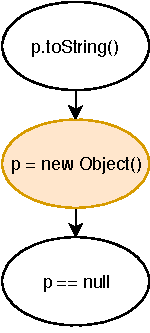
\includegraphics[]{figure/cfg-with-assignment-native.pdf}
\end{figure}

Figure \ref{figure:cfg-with-assignment-native} shows an typical example: in this case, we do not need to know what the native node (orange node) is exactly, but that the node assign \emph{p}. We do not care what exactly happen in this native node, we just need to know that, at one point, \emph{p} is assigned, even if in fact it is possible that the assignment is never executed. If it is the case, this will add false negative, but intuitively, we can assume that dead code is not common and this will not happen very often.

So, at this point, we know that we need to keep the content of the native nodes. 
The next step is to define what to do with them. 
A naive solution would be to add the content of the graph in the elements of the basic block, with the assumption that the evaluation order is not important. 
This is in fact correct for a native node with only one children, where the evaluation order can obviously not change. 
Here, we make the assumption that all the statements that change the flow of a program are represented in \slang{}. 
This is a reasonable assumption since programming language hardly ever provides exceptional statement that are break the control flow, and if it does, we can add it to \slang{} grammar.

\lstinputlisting[label={lst:ternary-expression-example},
caption=Pseudo code with a ternary expression]{code/ternary-expression-example.scala}

\begin{figure}[h]
	\caption{Basic block content of the code in listing above}
	\label{figure:basic-block-content}
	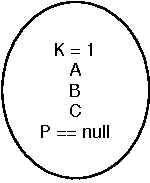
\includegraphics[]{figure/basic-block-content.pdf}
\end{figure}


Listing \ref{lst:ternary-expression-example} shows the pseudo code of a Java program with the control flow graph of the naive implementation in figure \ref{figure:basic-block-content}.
Since the ternary expression will be mapped to a native node in \slang{}, if we take the children of the native node in order, we will obtain the execution order of of the nodes in figure \ref{figure:basic-block-content}, that is obviously not correct, as the pointer will be seen as used then checked in this order, but not in the real execution order.

\begin{figure}[h]
	\caption{CFG with elements coming from natives nodes}
	\label{figure:two-unreliable-cfg}
	\setlength{\tabcolsep}{24pt}
	\begin{tabular}{cc}
		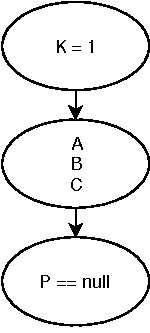
\includegraphics[]{figure/unreliable-cfg-1.pdf}  &
		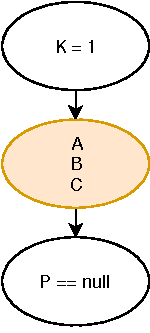
\includegraphics[]{figure/unreliable-cfg-2.pdf}   \\ 
		Splitted CFG & Splitted block with unreliable node
	\end{tabular}
\end{figure}

The idea to solve the problem showed before is to put all elements that comes from a native node in a separate basic block (figure \ref{figure:two-unreliable-cfg}, left), and mark it as \emph{unreliable} (figure \ref{figure:two-unreliable-cfg}, right), shown in orange. 
All control flow statement nested inside the native nodes will also lead to unreliable basic block.\newline
[Ev: show nested control flow nodes that are also unreliable]. 
Additionally, we will also mark the whole graph as unreliable. 

This information can now be used by any checker that use a control flow graph, not only for the null pointer dereference checker.

\subsubsection{How to use this information?}
\label{subsubsec:use_unreliable_information}

This information can be used in different ways to help to define the multiple level of granularity of the implementation of a new checker:

\begin{enumerate}
\item \textit{Ignore this information} \newline
In some case, it may make sense to simply ignore this information, and to treat unreliable nodes as others. 
In our case, we have shown previously that this solution is not suitable, as it produces too many false positives. \newline

\item \textit{Don’t run the checker on unreliable CFG} \newline
This is the opposite of the previous point: in the case where the checker need to really trust the control flow graph, it can make sense to simply stop the checker if the graph can not be trusted.

\begin{table}[h]
	\centering
	\caption{Percentage of native and completely native nodes in the different languages}
	\label{table:slang-native-percentage}
	\begin{tabular}{|c|c|c|c|}
		\hline
		\bf Language & \bf \% & \bf \% of completely native & \bf Number of files \\ \hline
		Scala &  41 &  6.25 & 6126 \\ 
		Kotlin &  47 &  6.5 & 26758 \\ 
		Ruby &  39 &  5.2 &  7811 \\ \hline
	\end{tabular}
\end{table}

Table \ref{table:slang-native-percentage} show the percentage of native nodes in \slang{} after translating open-source projects \cite{SlangSources:2019:Online} to \slang{}. The percentage of completely native nodes refers to the nodes that have all their children that are native. If more than $40\%$ of nodes are not translated, this does not mean that our language lack of information, because we do not mapped some kind of nodes on purpose.
This table shows us that natives nodes are not rare, using the above approach will greatly reduce our chance to find any relevant issue as we will in the majority of the case, be in the presence of natives nodes in the body of a function.

The two approach described before seems not well-suited for our checker, we may want something between the two extremes.

\item \textit{Fine grain} \newline
We can use the fact that we know if an element comes from a native node or not to define a finer grain implementation of our checker. 
It consist mainly in one modification of the data flow analysis described previously: we do not add a pointer that is used in an unreliable block to believed to be non-null set.

\begin{equation}\label{eqn:new_dataflow4}
newGen(n) = \text{use of pointer in the node n except if the node is marked as unreliable}
\end{equation}

\lstinputlisting[label={lst:fine-grain-1},
caption=First example of finer grain behaviour]{code/fine-grain-1.scala}

\lstinputlisting[label={lst:fine-grain-2},
caption=Second example of finer grain behaviour]{code/fine-grain-2.scala}

With this idea, we are now avoiding to report any issue for the two correct pseudo code from listing \ref{lst:fine-grain-1} and \ref{lst:fine-grain-2}. Since ternary expression are unreliable, we will not consider p as used, even though it may look like in the control flow graph.

\lstinputlisting[label={lst:fine-grain-3},
caption=Third example of finer grain behaviour]{code/fine-grain-3.scala}

In listing \ref{lst:fine-grain-3} though, the real evaluation order use \emph{p} and then check it for null. This code is not reported by our tool despite the fact that it should be. This is a false negative.\newline

\lstinputlisting[label={lst:fine-grain-4},
caption=Fourth example of finer grain behaviour]{code/fine-grain-4.scala}

In addition, the implementation will  still report issues inside native nodes.
For example, in listing \ref{lst:fine-grain-4}, we can see that the pointer \emph{p} is used, and then checked for null later in a un-trusted node. We do not know exactly what exactly happen in this node, but we can expect that a check for null still mean that p can be null. 
In this example, we report a true positive.
\end{enumerate}

\subsection{Other problematic situations}
\label{subsec:other_problematic_situation}
	
We have already presented the main problematic situations, coming form native nodes, but there is still a few cases that can raise false positive that we have to take care.

\subsubsection{Boolean short-circuit}
\label{subsubsec:boolean_short_circuit}

Our current implementation of the control flow graph does not encode the possible path due to Boolean short-circuit. 
This will in fact lead to a wrong evaluation order, even if the nodes are known. 
Since the evaluation order is not correct, it makes sense to treat them the same way we do with native nodes! 
We will hence keep all the content of these nodes, to be able to use them in the checkers, but mark them as unreliable. 

\lstinputlisting[label={lst:boolean-short-circuit},
caption=Problematic situation due to Boolean short circuit]{code/boolean-short-circuit.scala}

With this addition, we are now able to avoid the false negative that were reported in the well-known example of listing \ref{lst:boolean-short-circuit}.

\subsubsection{Order of evaluation of known nodes}
\label{subsubsec:evaluation_known_nodes}

In section \ref{how_to_deal_with_native}, we have seen that the order of evaluation of the nodes are critical for our checker.
When coming from different languages, even known nodes can have different evaluation order, as we have seen an example in section \ref{match_tree_cfg}. 
The same situation can in fact arise for any statement, hopefully, the solution is often to add the support for the new behavior in \slang{}.
This trick should be used with caution, the initial goal is to be language agnostic, we should ideally not have to modify \slang{} for every new language we add. The good news is that there is only a limited number of possible variations that are possible, since the number of known nodes is fixed (and only a faction of it in practice). 
This kind of problem is a difficulty that are hard to anticipate and will arise during the implementation of a new checker, but it is not in itself a strong limitation.

\subsubsection{Lost Jump Statements}
\label{subsubsec:lost_jump_statement}

We have seen in section \ref{subsubsec:jump_tree_cfg} that we add the jump statement to the basic block if we do not expect it, without doing anything special.
In fact, we face a similar uncertainties that happen with natives nodes, we do not know exactly what is happening, but we can expect that something will go wrong. 
The same happen with jump tree with label, as the way the different language deals with label can be arbitrary, we can not assume anything. 
We just know that the statement will change the execution flow in an unreliable way, we will therefore mark the flow generated as \emph{unreliable}.

